\documentclass{article}

\title{Homework 1 : Graphs and Network Flows}
\author{Aashith Kamath Manjeshwar, Saikrishna Badrinarayanan}
\newcommand{\R}{\mathbf{R}}
\newcommand{\U}{\mathbf{U}}
\newcommand{\m}{\mathsf{m}}
\newcommand{\M}{\mathsf{M}}
\usepackage{hyperref}

\usepackage{graphicx}
\graphicspath{ {plots/} }
\begin{document}
\maketitle

In this project, we use the igraph library to study several properties of 
real networks available at \url{https://www.dropbox.com/s/oybns7fvztfy76q/sorted_directed_net.txt?dl=0}. We use 
the netrw package to run random walks on the graphs
generated. The project was coded in the language R.

\paragraph{Problem 1}: \\
We first check whether the given network is connected. It turns out that it's \textbf{not connected}.
We then compute the Giant Connected Component (GCC) of the network. The GCC of a graph is
a connected component that contains a constant fraction of the entire graph’s
vertices. We find the GCC by first computing the set of clusters in the graph
and then the largest cluster among them. We then delete the vertices that do
not belong to the largest cluster and this gives the GCC. In all the problems from now, we work 
with the GCC of the network.\\

\hrule

\paragraph{Problem 2}:\\
In this problem, we measure the degree distribution of the in-degree and out-degree of the nodes.
The degree distribution is a plot containing the various degrees of the nodes in the graph on the x-axis
and their corresponding density (frequency of that degree occuring divided by the total number of nodes) on the y-axis.\\
\pagebreak

\textbf{In-degree}\\
The x-axis contains the in-degree and y-axis the corresponding density.\\
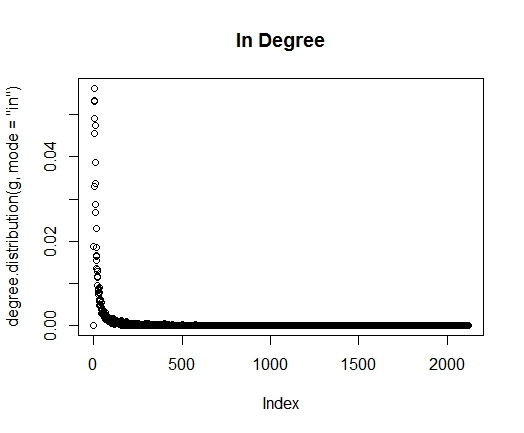
\includegraphics[scale=0.4]{p1} \\
\textbf{Out-degree}\\
The x-axis contains the out-degree and y-axis the corresponding density.\\
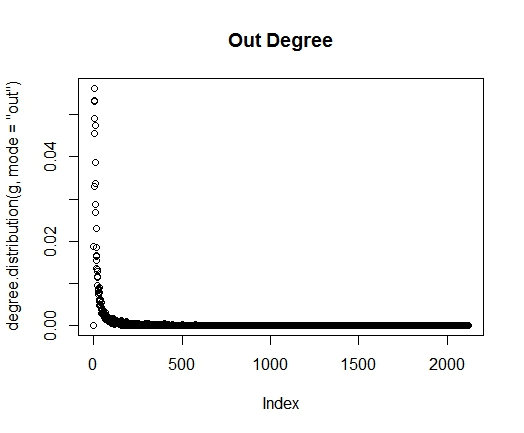
\includegraphics[scale=0.4]{p2} \\
Surprisingly, both the degree distributions looks identical.\\

\hrule

\paragraph{Problem 3}:\\
In this question, we measure the community structure of the network. 
A network is said to have a community structure if the nodes of the network 
can be easily grouped into (potentially overlapping) sets of nodes such that each set is densely connected internally. 
We use two methods - \textit{fastgreedy.community} and \textit{label.propagation.community}.
The first step is to convert the directed graph into an undirected graph retaining all the properties. This is because
the two methods to find community structure listed above work only on undirected graphs. The transformation from
directed to undirected is non-trivial due to the presence of edge weights. We consider two approaches to achieve this transformation.
\begin{itemize}
 \item \textbf{Option 1 :}\\
 We simply convert every directed edge into an undirected one retaining the same weight.
 This is done using the ``as.undirected'' function and invoking the ``each'' parameter.
 Here, the number of edges in the graph remains unchanged. 
 We find the community structure of the graph only using the 
 label.propagation.community method. (The question explicitly mentions only this method for this option. We realized 
 that with the other method it wouldn't work as fastgreedy.community requires every pair of vertices to have only a single
 edge between them which wouldn't be the case here.) The figure below contains
 the community structure using label.propagation.community. The x-axis denotes the sizes of the communities obtained
 and the y-axis denotes the number of communities with that size.\\
 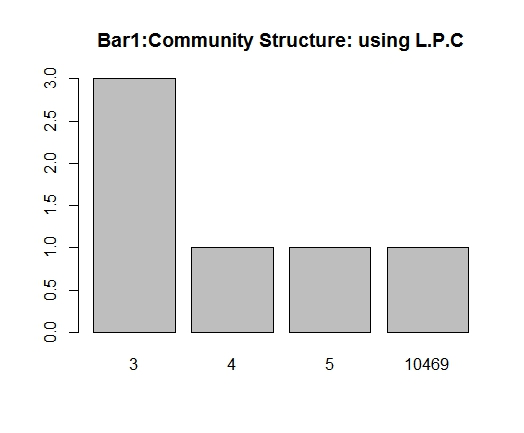
\includegraphics[scale=0.4]{p3} 
 \item \textbf{Option 2 :}\\
 Here, we take the set of directed edges between any pair of nodes and combine them into a single undirected edge.
 This is done using the ``as.undirected'' function and invoking the ``collapse'' parameter.
 The weight of the resulting edge is the square root of the product of all the edges that get combined. We initially toyed 
 with the idea of also taking the $n^{th}$ root of the product if we were combining $n$ directed edges into one.
 However, we decided to not explore that option further and stuck only to the square root approach. We just give a theoretical
 observation that the $n^{th}$ root method is another alternate.
 Note that in this option, we can find the community structure using fastgreedy.community too as we have only a single
 edge between every pair of vertices.\\
 
 The first figure drawn below contains the community structure using label.propagation.community. The x-axis denotes the sizes of the communities obtained
 and the y-axis denotes the number of communities with that size.\\
 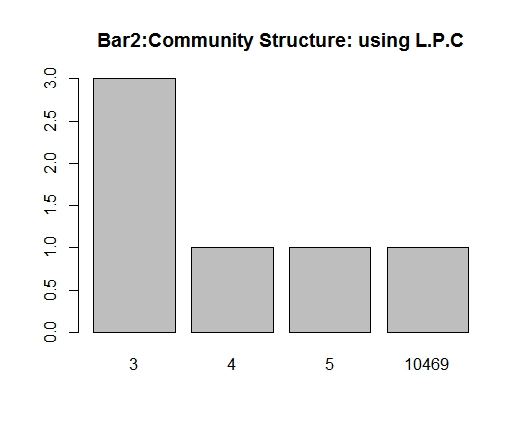
\includegraphics[scale=0.4]{p4}\\
 The next figure contains the community structure using fastgreedy.community. The x-axis denotes the sizes of 
 the communities obtained and the y-axis denotes the number of communities with that size.\\
 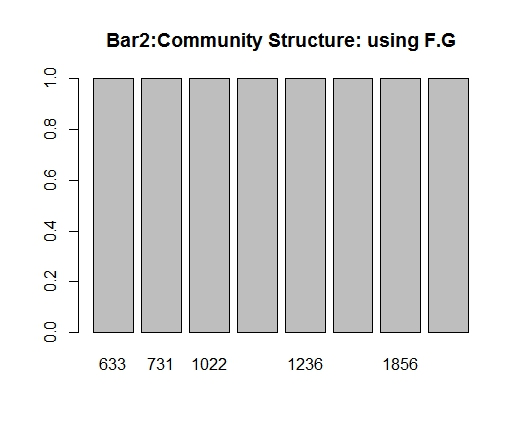
\includegraphics[scale=0.4]{p5} 
\end{itemize}
\textbf{Comparison :}\\
In case of label.propagation.community, the community structure obtained is the same using either of the two options in
transforming the graph from directed to undirected.\\
In the second transformation option, where we find the community using both the methods, the resulting community structures
are quite different. Using fastgreedy, the sizes of the communities are much larger and the frequency is 1 for each size.
The number of communities is 8.
Using label.propagation, the sizes of the communities are much smaller (except for one of them which is extremely large), and 
the smallest size has a frequency of 3 while the rest have a frequency of 1. The number of communities (6) is also lesser.\\

\hrule

\paragraph{Problem 4}:\\
We find the largest community computed above from fastgreedy.community (using option 2). We isolate this community
to form a new network and find the community structure of this new network. We call this the sub-community structure
of the largest community. 
 The figure below contains the community structure. The x-axis denotes the sizes of the communities obtained
 and the y-axis denotes the number of communities with that size.\\
 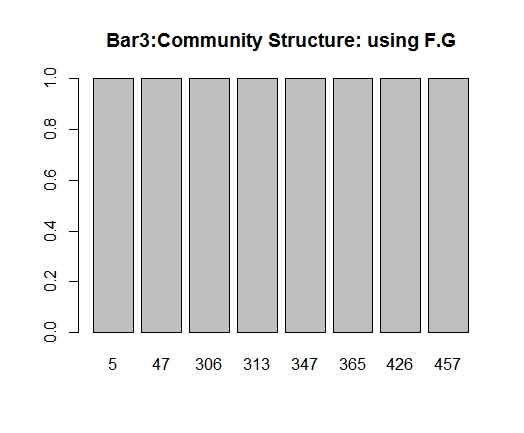
\includegraphics[scale=0.4]{p6}\\
 We try to repeat the same thing using label.propagation.community and the results as expected aren't very good.
 This is because, using label.propagation method, the size of the largest community is 10469 nodes, which contains
 almost the entire given network. The community structure of the new network obtained from this community is 
 essentially the whole community again. That is, it gives only one community of size 10469. The result was expected
 but we just tried it for the sake of completeness. The plot is shown below.\\
 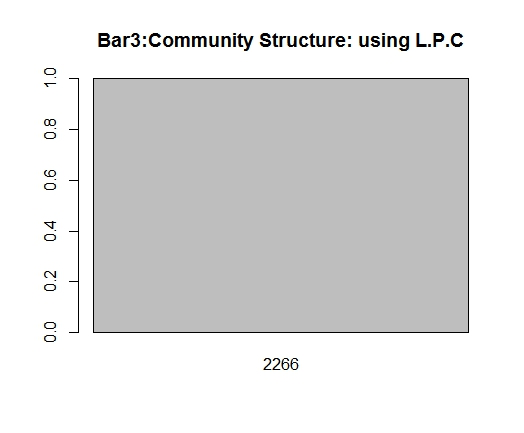
\includegraphics[scale=0.4]{p7}\\
 
 \hrule
 
\paragraph{Problem 5}:\\
In the community structure we find using fastgreedy.community in problem 3, we first find all the communities with 
size greater than 100. Then, for each of these communities we find it's sub-community structure. 
As in the previous problem, The sub-community structure of a given community is the community structure obtained
by isolating this community from the rest of the network and treating it as a net network.
We observe that there are 8 communities with size larger than 100. Their sizes and sub-community structures are shown below:\\
\begin{enumerate}
 \item 
 Size : 1856.\\
 The figure below contains the community structure. The x-axis denotes the sizes of the communities obtained
 and the y-axis denotes the number of communities with that size.\\
 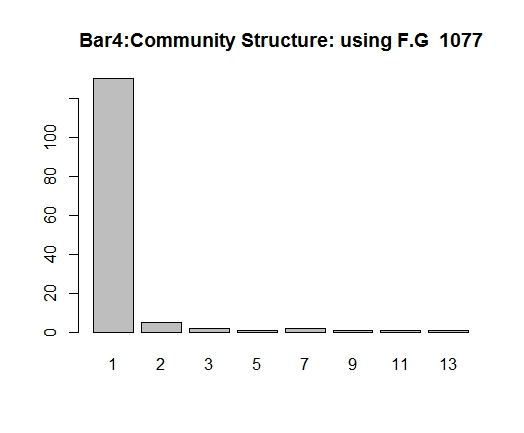
\includegraphics[scale=0.4]{p8}

 \item 
 Size : 1666.\\
 The figure below contains the community structure. The x-axis denotes the sizes of the communities obtained
 and the y-axis denotes the number of communities with that size.\\
 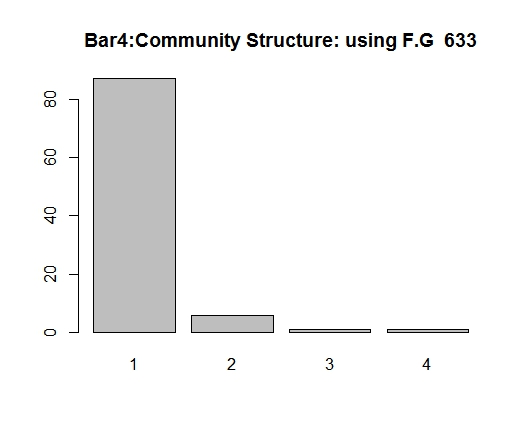
\includegraphics[scale=0.4]{p9}
 
 \item 
 Size : 1022.\\
 The figure below contains the community structure. The x-axis denotes the sizes of the communities obtained
 and the y-axis denotes the number of communities with that size.\\
 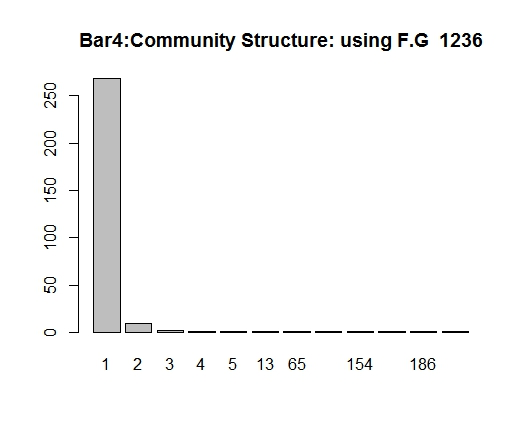
\includegraphics[scale=0.4]{p10}
 
 \item 
 Size : 2266.\\
 The figure below contains the community structure. The x-axis denotes the sizes of the communities obtained
 and the y-axis denotes the number of communities with that size.\\
 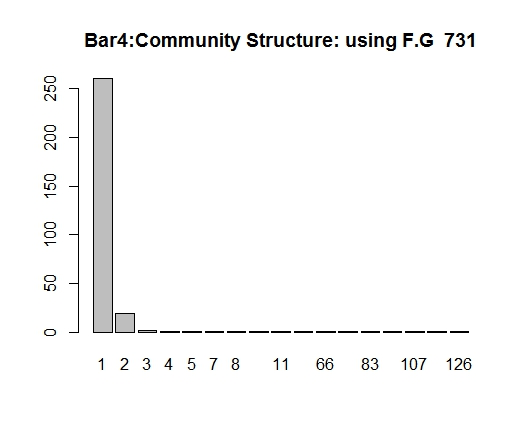
\includegraphics[scale=0.4]{p11}
 
 \item 
 Size : 731.\\
 The figure below contains the community structure. The x-axis denotes the sizes of the communities obtained
 and the y-axis denotes the number of communities with that size.\\
 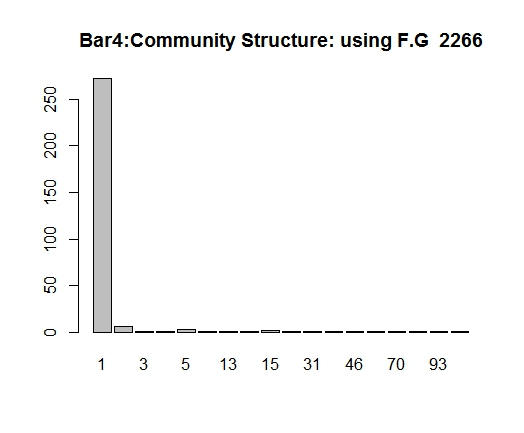
\includegraphics[scale=0.4]{p12}
 
 \item 
 Size : 1236.\\
 The figure below contains the community structure. The x-axis denotes the sizes of the communities obtained
 and the y-axis denotes the number of communities with that size.\\
 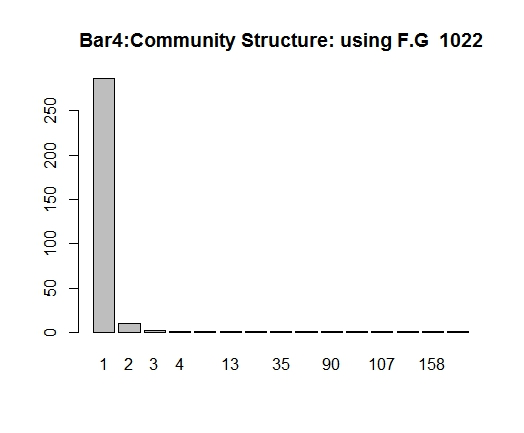
\includegraphics[scale=0.4]{p13}
 
 \item 
 Size : 633.\\
 The figure below contains the community structure. The x-axis denotes the sizes of the communities obtained
 and the y-axis denotes the number of communities with that size.\\
 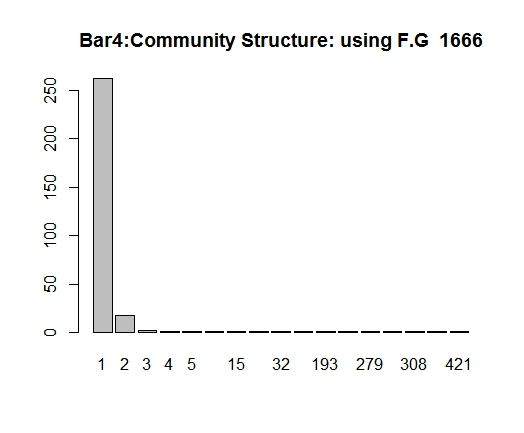
\includegraphics[scale=0.4]{p14}
 
 \item 
 Size : 1077.\\
 The figure below contains the community structure. The x-axis denotes the sizes of the communities obtained
 and the y-axis denotes the number of communities with that size.\\
 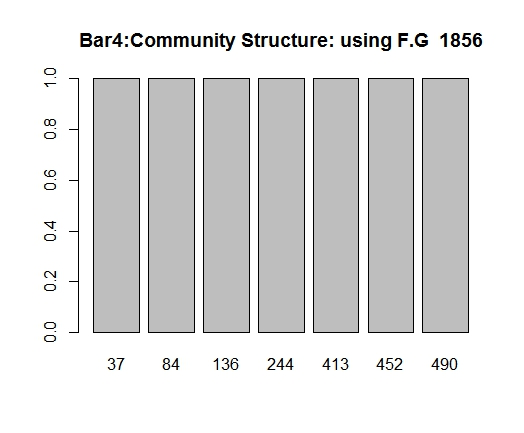
\includegraphics[scale=0.4]{p15}

 
 
 \end{enumerate}

 \hrule
 
\paragraph{Problem 6}:\\
In this problem, the goal is to find the number of communities each node belongs to. In all the above methods,
we only get 1 community that each node belongs to. However, in practice, a node can be a part of several communities and 
the igraph package cannot detect overlapping communities. In order to compute this, we use the notion of personalized pagerank.
We start at each node and perform a random walk by setting the damping parameter to be $0.85$. We use this information
along with the community structure computed earlier to find the number of communities for each node.\\

More concretely, let's consider a node $i$. We perform a random walk starting at $i$ on the original directed network
by setting the damping parameter to be $0.85$. We simulate the random walk using 10 walkers and perform 1000 steps for each
walker. In the random walk, we set the teleportation probability to be 1 for the starting node and 0 for other 
nodes. That is, at each time step, if the walk decides to teleport and not move to a neighbour (which happens with probability
$0.15$), it always teleports back to the starting node.
At the end of the walk, we calculate the average visit probability for each node from node $i$.
Then, we calculate the vector $\vec{\M}_i$ in the following manner:\\
$$\vec{\M}_i = \Sigma_j v_j\vec{\m}_j$$
where $v_j$ is the visit probability for node $j$ and $\vec{\m_j}$ is the membership vector for node $j$.\\
Suppose the number of communities computed using the previous method is $n$.
The membership vector for a node $j$ has $n$ elements where every index has value 0 except for the index
corresponding to the community to which $j$ belongs to, which has value $1$.
Thus, $\vec{\M}_i$ is a $n$ dimensional vector.\\

In our computation using the fastgreedy method to find the community structure, the number of communities is 8 and so the 
value of $n$ is 8. We don't consider the label.propagation method because the community structure it outputs is pretty skewed.
That is, it has 1 community that contains the majority of the nodes and a few other very small communities. So, we believe that such
an analysis to find overlapping communities would be futile and not very accurate in that case and hence we stick
to finding multiple communities that each node could exist in using the fastgreedy method only.\\

Further, since the number of nodes is very large and the visit probability for a large fraction of them would be very small,
we make the process more efficient by considering only 30 nodes in the summation, corresponding to the top 30 visit
probabilities. Thus, to summarize, we calculate an 8-dimensional vector $\vec{M}_i$ for each node $i$ by summing up 
the product of the visit probability $v_j$ and the membership vector $\vec{m}_j$ for the 30 nodes with the highest average visit
probability when starting a random walk from node $i$.\\

Finally, we set a certain threshold $t$. Now, for each node $i$, we count the number of entries of $\vec{\M}_i$ that 
are above the threshold and say that node $i$ belongs to all those communities. In this problem, our goal is to only list 
atleast 3 nodes that are present in multiple communities. After a careful analysis of the observed vectors $\vec{\M}_i$,
we choose the threshold to be $0.45$. Using this threshold value, we find the following nodes to be in multiple communities :
$10441,10442,10470,10471,10478,10479$. All of them are present in two communities each.
When we set the threshold to be $0.18$, we get 19 nodes in multiple communities. From $0.2$
onwards, the above are the only 6 nodes in multiple communities.\\

Now, we repeat the whole analysis by using the GCC of the directed graph for performing the random walk and 
not the original graph itself. For a threshold value of $0.15$, there are no nodes present in multiple communities.
There are 6 nodes present in two communities when the threshold is $0.14$. When we choose the threshold to be
$0.145$, there are three nodes present in two communities each. The nodes are $6205,9784$ and $10151$. 
Further, we also
observe that one of the two communities they belonged to was actually the original community that they were reported
to belong to as per the result of the fastgreedy algorithm. Also, the value in that index in their $\vec{M}$ was the 
highest among the 8 values. This is not surprising because we would expect the community detection algorithms which
report only 1 community per node (like the fastgreedy) to place each node in the most probable community for it.
\begin{itemize}
 \item \textbf{Node 6205}\\
 Community number from Fastgreedy : 8\\
 Our analysis : 2, 8
 
 \item \textbf{Node 6205}\\
 Community number from Fastgreedy : 8\\
 Our analysis : 2, 8
 
 \item \textbf{Node 9784}\\
 Community number from Fastgreedy : 7\\
 Our analysis : 1, 7
 
 \item \textbf{Node 10151}\\
 Community number from Fastgreedy : 4\\
 Our analysis : 1, 4
\end{itemize}
Note, here we have numbered the communities from 1 to 8 in the same order in which they were plotted in the x-axis
of the community structure plot in problem 3.\\

We repeated the same experiment without setting the teleportation probabilities. That is, at each step,
if the walk decides to teleport, it now teleports to a random node. In this case, we observe that for threshold 
values in the range $0.3$ to $0.4$, there are several nodes (around 20) present in multiple communities. However,
even if we set the threshold to be $0.05$, there isn't even a single node present in more than 1 community.


\end{document}
